% !TeX root = ../index.tex
\chapter{Development}
% 25 marks

\fxerror{Not started}

\section{Requirements Elicitation}

\section{API}

\begin{enumerate}
  \item It should only store the data necessary to function
    \begin{itemize}
      \item Users: id
      \item Library Entries: ratings, completion status and episode progress
      \item Anime: airing status, episode count and start date
    \end{itemize}
  \item It should store all active Kitsu users
  \item It should store all library entries linked to users
  \item It should only store anime if they have at least one library entry linked to it
  \item It should continuously update the data stored at a regular interval
  \item It should output the user and anime stats:
    \begin{itemize}
      \item total number of library entries
      \item mean, median and mode ratings
      \item the variance and standard deviation of the ratings
      \item the raw rating frequencies
    \end{itemize}
  \item It should output the user and anime stats by the year an anime started airing
  \item It should output the user and anime stats by the categories anime are a part of
  \item It should output the total episodes a user has seen
\end{enumerate}

\section{API Consumption}

\begin{enumerate}
  \item It should allow the user to enter a user or anime to find stats for
  \item It should display the stats provided by the API (see 6-9 above)
\end{enumerate}

\section{Design}

\begin{figure}[H]
  \caption{API user stats}
  \centering
  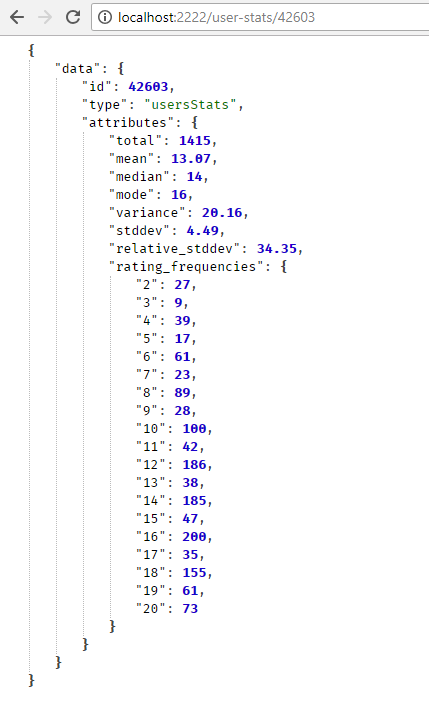
\includegraphics[width=.6\textwidth]{6-user}
\end{figure}

\begin{figure}[H]
  \caption{API user stats with null values}
  \centering
  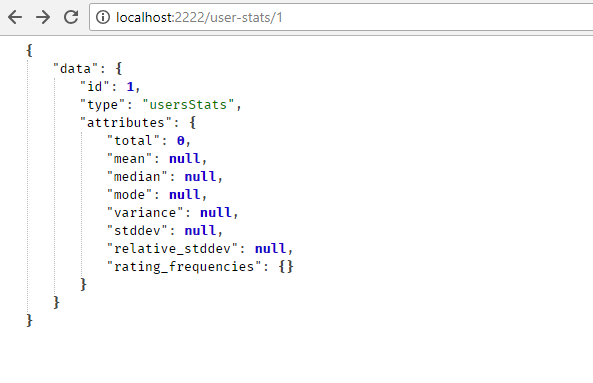
\includegraphics[width=.75\textwidth]{6-user-null}
\end{figure}

\begin{figure}[H]
  \caption{API anime stats}
  \centering
  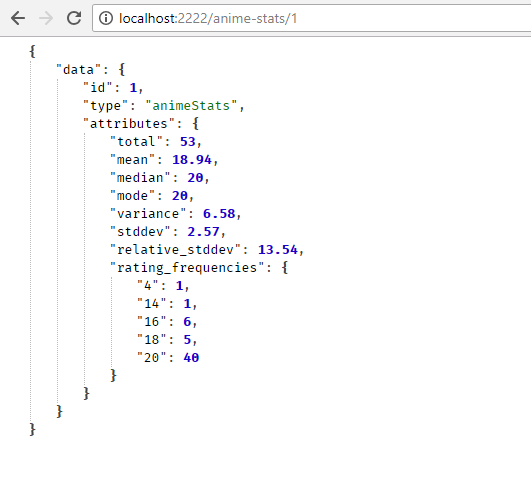
\includegraphics[width=.75\textwidth]{6-anime}
\end{figure}

\section{Implementation}

A working example of the implementation can be viewed at \url{https://api.hibari.moe/} with the following URLs:

\begin{itemize}
  \item \url{https://api.hibari.moe/user-stats/42603}
  \item \url{https://api.hibari.moe/anime-stats/1}
\end{itemize}

\subsection{Kitsu API Proxy}

I included a simple proxy of the Kitsu API, which passes the request to Kitsu and returns the response. This is beneficial as the Kitsu API does not serve its responses with gzip compression, so responses are considerably larger. As a result the proxy requests for end-users are only a few kilobytes to download instead of several hundred with subsequent requests to the same URI being almost instant, with no external request to Kitsu's API, thanks to memory caching on the production server which caches requests for 15 minutes.

\captionsetup{type=figure}\captionof{figure}{src/routes/proxy.cr}
\subfile{pyg/src/routes/proxy}

\newpage
\subsection{Kitsu API Requests}

All requests to the Kitsu API go through this method which returns a string to the calling method.

\captionsetup{type=figure}\captionof{figure}{src/kitsu/get.cr}
\subfile{pyg/src/kitsu/get}

\newpage
\subsection{Calculating The Stats}

The stats used for the user and anime endpoints are implemented into the Array data type's class. This allows generating the statistics by doing \texttt{mystats.mean} instead of creating module-namespaced methods that accepted an array of integers (e.g \texttt{Stats.mean mystats})

\captionsetup{type=figure}\captionof{figure}{src/stats/stats.cr}
\subfile{pyg/src/stats/stats}

\newpage
\subsection{Anime \& User Stats Generation}

Stats generation involves querying the database for all library entries for the given user or anime (two separate methods). This is then mapped to an integer array of user ratings.

Stats are then added to a Hash (\texttt{stats}) which is returned by the method.

\captionsetup{type=figure}\captionof{figure}{src/stats/user\_stats.cr}
\subfile{pyg/src/stats/user_stats}

\newpage
\subsection{Anime \& User Stats Output}

Using the above method, the stats are then output from the API through a route in the Kemal framework. The user (or anime) is queried. If the user doesn't exist in the database, a 404 error is thrown (see \url{src/json_api/error.cr} for the \texttt{Hibari::JsonAPI.error} implementation). The JSON response is then built using the standard library with some helper functions for code-reuse and reducing the amount of nesting.

\captionsetup{type=figure}\captionof{figure}{src/routes/user-stats.cr}
\subfile{pyg/src/routes/user-stats}

\newpage
\captionsetup{type=figure}\captionof{figure}{src/json\_api/field.cr}
\subfile{pyg/src/json_api/field}

\captionsetup{type=figure}\captionof{figure}{src/json\_api/attribute\_stats.cr}
\subfile{pyg/src/json_api/attribute_stats}

\newpage
\subsection{Populating the Database}

The database is populated on a schedule that is run every Sunday. This first inserts, or updates, users into the database. It then fetches all of the user IDs in the database and fetches their library entries. Library entries and anime are inserted/updated simultaneously to reduce the amount of requests needed to be sent to the Kitsu API.

The Kitsu API has a maximum resources-per-page limit of 500 for library entries, while fetching anime using its own endpoint has a limit of 20. By using the relationship functionality of JSON:API I can include the anime data when requesting the library entries. This reduces the requests needed by 25 times.

\captionsetup{type=figure}\captionof{figure}{src/cron/index.cr}
\subfile{pyg/src/cron/index}

\newpage
\captionsetup{type=figure}\captionof{figure}{src/cron/tasks/users.cr}
\subfile{pyg/src/cron/tasks/users}

\newpage
\captionsetup{type=figure}\captionof{figure}{src/cron/helpers/create\_user.cr}
\subfile{pyg/src/cron/helpers/create_user}

\newpage
\captionsetup{type=figure}\captionof{figure}{src/cron/tasks/library\_entries.cr}
\subfile{pyg/src/cron/tasks/library_entries}

\newpage
\captionsetup{type=figure}\captionof{figure}{src/cron/helpers/create\_anime.cr}
\subfile{pyg/src/cron/helpers/create_anime}

\newpage
\captionsetup{type=figure}\captionof{figure}{src/cron/helpers/create\_library\_entries.cr}
\subfile{pyg/src/cron/helpers/create_library_entries}

\newpage
\subsection{Database Models}

The database models for interfacing with the SQLite database in Crystal using the Crecto shard (\url{https://github.com/Crecto/crecto})

\captionsetup{type=figure}\captionof{figure}{src/repo/models/models.cr}
\subfile{pyg/src/repo/models/models}
